


\begin{applicationActivities}{4}{10}

\begin{fact}
  At least \(n\) vectors are required to span \(\IR^n\).

  \begin{center}
  \begin{tikzpicture}[scale=0.5]
    \draw[<->] (-4,0) -- (4,0);
    \draw[<->] (0,-4) -- (0,4);
    \draw[blue!50] (2,-4) -- (-2,4);
    \draw[thick,blue,->] (0,0) -- (1,-2);
  \end{tikzpicture}
  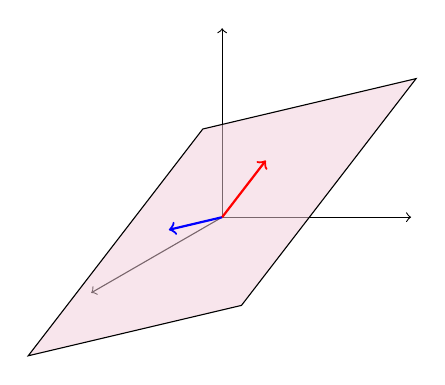
\begin{tikzpicture}[x={(210:0.8cm)}, y={(0:1cm)}, z={(90:1cm)},scale=0.4]
    \draw[->] (0,0,0) -- (6,0,0);
    \draw[->] (0,0,0) -- (0,6,0);
    \draw[->] (0,0,0) -- (0,0,6);
    \draw[fill=purple!20,fill opacity=0.5]
      (-2,-2,2) -- (6,-2,-2) -- (2,2,-2) -- (-6,2,2) -- (-2,-2,2);
    \draw[thick,blue,->] (0,0,0) -- (1,-1,0);
    \draw[thick,red,->] (0,0,0) -- (-2,0,1);
  \end{tikzpicture}
  \end{center}
\end{fact}

\begin{activity}{10}
  Choose a vector \(\begin{bmatrix}a\\b\\c\end{bmatrix}\)
  in \(\IR^3\) that is not in
  \(\vspan\left\{\begin{bmatrix}1\\-1\\0\end{bmatrix},
  \begin{bmatrix}-2\\0\\1\end{bmatrix}\right\}\) by ensuring
  \(\begin{bmatrix}[cc|c]1&-2&a\\-1&0&b\\0&1&c\end{bmatrix}\sim
  \begin{bmatrix}[cc|c]1&0&0\\0&1&0\\0&0&1\end{bmatrix}\).
  (Why does this work?)
\end{activity}

\begin{fact}
  The set \(\{\vect v_1,\dots,\vect v_m\}\) fails to span all of \(\IR^n\)
  exactly when \(\RREF[\vect v_1\,\dots\,\vect v_m]\) has a row of zeros:
  \[\begin{bmatrix}[cc]1&-2\\-1&0\\0&1\end{bmatrix}\sim
  \begin{bmatrix}[cc]1&0\\0&1\\0&0\end{bmatrix}\Rightarrow
  \begin{bmatrix}[cc|c]1&-2&a\\-1&0&b\\0&1&c\end{bmatrix}\sim
  \begin{bmatrix}[cc|c]1&0&0\\0&1&0\\0&0&1\end{bmatrix}\]
\end{fact}

\begin{activity}{5}
  Consider the set of vectors \(S=\left\{
  \begin{bmatrix}2\\3\\0\\-1\end{bmatrix},
  \begin{bmatrix}1\\-4\\3\\0\end{bmatrix},
  \begin{bmatrix}2\\0\\0\\3\end{bmatrix},
  \begin{bmatrix}0\\3\\5\\7\end{bmatrix},
  \begin{bmatrix}3\\13\\7\\16\end{bmatrix}
  \right\}
  \).
  Does
  \(\IR^4=\vspan S\)?
  % \begin{subactivity}
  % Find a linear combination of vectors in \(S\) that equals
  % \(\begin{bmatrix}-1\\10\\7\\14\end{bmatrix}\).
  % \end{subactivity}
\end{activity}

\begin{activity}{10}
  Consider the set of third-degree polynomials \[S=\left\{
  2x^3+3x^2-1,
  2x^3+3,
  3x^3+13x^2+7x+16,
  -x^3+10x^2+7x+14,
  4x^3+3x^2+2
  \right\}
  .\]
  Does
  \(\P^3=\vspan S\)?
  % \begin{subactivity}
  % Find a vector in \(\IR^4\) that is not in \(\vspan S\).
  % \end{subactivity}
\end{activity}

\begin{definition}
  A subset of a vector space is called a \term{subspace} if it is
  itself a vector space.
\end{definition}

\begin{fact}
  If \(S\) is a subset of a vector space \(V\), then
  \(\vspan S\) is a subspace of \(V\).
\end{fact}

\begin{remark}
  To prove that a subset is a subspace, you need only verify that
  \(c\vect v+d\vect w\) belongs to the subset for any choice of
  vectors \(\vect v,\vect w\) from the subset and any real scalars \(c,d\).
\end{remark}

\begin{activity}{5}
  Prove that \(P=\{ax^2+b:a,b\text{ are both real numbers}\}\) is a subspace
  of the vector space of all degree-two polynomials by showing that
  \(c(a_1x^2+b_1)+d(a_2x^2+b_2)\) belongs to \(P\).
\end{activity}

\begin{activity}{10}
  Consider the subset of \(\IR^2\) where at least one coordinate of
  each vector is \(0\).
  \begin{center}
    \begin{tikzpicture}[scale=0.25]
    \draw[thin,gray,<->] (-5,0) -- (5,0);
    \draw[thin,gray,<->] (0,-5) -- (0,5);
    \draw[thick,blue] (-4.8,0) -- (4.8,0);
    \draw[thick,blue] (0,-4.8) -- (0,4.8);
    \end{tikzpicture}
  \end{center}
  % \begin{subactivity}
    Find a linear combination
    \(c\vect v+
    d\vect w\) that does not
    belong to this subset.
  % \end{subactivity}
  \begin{TBLnote}
    Use this linear combination to sketch a picture
    illustrating why this subset is not
    a subspace.
  \end{TBLnote}
\end{activity}

\begin{fact}
  Suppose a subset \(S\) of \(V\) is isomorphic to another vector space
  \(W\).
  Then \(S\) is a subspace of \(V\).
\end{fact}

\begin{activity}{5}
  Show that the set of \(2\times 2\) matrices
  \[S=
    \left\{
    \begin{bmatrix}a&b\\-b&-a\end{bmatrix} :
    a,b\text{ are real numbers}
    \right\}
  \]
  is a subspace of \(\IR^{2\times 2}\) by identifying a Euclidean
  space isomorphic to \(S\).
\end{activity}



\end{applicationActivities}
